\graphicspath{{8cardinality/asy/}}

\section{Cardinality and Infinite Sets}\label{chap:cantor}

During the late 1800's, Georg Cantor assaulted the foundations of mathematics with his investigations of certain infinite sets, in particular his middle-third set (Example \ref{ex:cantorthird}). Cantor's ideas about infinity met significant resistance: some mathematicians and philosophers considered his approach unnatural; he even inflamed religious scholars who thought his ideas an affront to the divine!\smallbreak

Despite initial skepticism, Cantor's notion of cardinality is now universally accepted. By unearthing several contradictions inherent in contemporary (naïve) set theory, mathematicians became convinced that a rigorous \emph{axiomatic} approach was necessary. Developing an axiomatic foundation to mathematics became a core goal of early 20\th{} century mathematics.


\subsection{Cantor's Notion of Cardinality}\label{sec:cantor}

Recall that the \emph{cardinality} $\nm A$ of a finite set $A$ is simply the number of elements of $A$ (Definition \ref{defn:card1}). While ``number of elements" is meaningless for infinite sets, cardinality also gives rise to a \emph{relation} $\le$ which can be used to \emph{compare} sets; this interpretation does extend to infinite sets\ldots

\begin{example}{}{}
	Consider two sets
	\[
		A=\{\text{fish},\text{dog}\}\qquad B=\{\alpha,\beta,\gamma\}
	\]
	While the elements of $A$ and $B$ are completely different, the sets themselves may be compared using cardinality: we write $\nm A\le \nm B$ to indicate that $B$ has at least as many elements as $A$. In Theorem \ref{thm:finitecard}, we saw that this mandates the existence of an \emph{injective function} $f:A\to B$: plainly
	\[
		f(\text{fish})=\alpha,\qquad f(\text{dog})=\beta
	\]
	defines a suitable function.
\end{example}

Theorem \ref{thm:finitecard} tells us how functions may be used to \emph{compare cardinalities} of finite sets \emph{without counting elements.} Cantor's seemingly innocuous idea was to turn this \emph{theorem} for finite sets into a general \emph{definition} of cardinality.


\begin{defn}{}{infcard}
	The \emph{cardinality} of a set $A$ is denoted $\nm A$. We compare cardinalities as follows:
	\begin{itemize}
  	\item $\nm A\le\nm B\iff\exists f:A\to B$ injective.
  	\item $\nm A=\nm B\iff\exists g:A\to B$ bijective.
	\end{itemize}
	$\nm A<\nm B$ means $\nm A\le \nm B$ and $\nm A\neq \nm B$, that is $\exists f:A\to B$ injective but $\nexists g:A\to B$ bijective.
\end{defn}

\begin{lemm}{}{cardequiv}
	Equality of cardinality $\nm A=\nm B$ is an equivalence relation on any collection of sets.
\end{lemm}

``Cardinality'' is an abstract property whereby sets can be \emph{compared}, rather than a \emph{value} attaching to a given set.\footnote{We \emph{could} use the Lemma to define $\nm A:=[A]$ as the equivalence class of $A$, though this likely feels confusing!} Regardless, the Lemma proves that cardinality partitions any collection of sets: every set has a cardinality, and no set has more than one cardinality. It is moreover natural to identify the cardinalities of finite sets with the \emph{cardinal numbers} $0,1,2,3,4,\ldots$

\goodbreak



\boldsubsubsection{Countably Infinite Sets}


To make progress, it is helpful to introduce a symbol for the cardinality of the simplest infinite set.

\begin{defn}{}{}
	We say that $A$ is a \emph{countably infinite\footnotemark} set and write $\nm A=\aleph_0$ (\emph{aleph-nought} or \emph{aleph-null}), if its cardinality equals that of the set of \emph{natural numbers} $\N$:
	\[
		\nm A=\aleph_0 \iff \exists g:\N\to A\text{ bijective}
	\]
\end{defn}

\footnotetext{%
	Some authors say \emph{denumerable} and use \emph{countable} for sets with $\nm A\le\aleph_0$. \emph{Aleph} is the first letter of the Hebrew alphabet.%
}

In the next section we'll see why a new symbol is necessary; why $\infty$ doesn't suffice.

\begin{examples}{}{easycantor}
	\exstart The function $g:\N\to\N_{\ge 2}$ defined by $g(n)=n+1$ is a bijection, whence $\N_{\ge 2}=\{2,3,4,5,\ldots\}$ is countably infinite.\footnotemark
	\begin{enumerate}\setcounter{enumi}{1}
	  \item Let $2\N=\{2,4,6,8,10,\ldots\}$ be the set of positive even integers. The function
		\[
			h:\N\to 2\N:n\mapsto 2n
		\]
		is a bijection. It follows that $\nm{2\N}=\nm\N=\aleph_0$ and that $2\N$ is countably infinite.
	\end{enumerate}
\end{examples}

\footnotetext{%
	This is a version of \emph{Hilbert's Grand Hotel Problem.} Imagine a hotel with an infinite number of rooms: Room 1, Room 2, Room 3, Room 4, etc. Even if the hotel is full, by moving everyone one room down the hall, space can always be found for an additional guest. The second example is another version, where infinitely many new guests may be accommodated!%
}

Theses examples demonstrate a perplexing property of infinite sets. For instance, $2\N$ is a \emph{proper subset} in bijective correspondence with $\N$! It feels like we want to say two contradictory things:
\begin{itemize}
  \item $\N$ has the `same number of elements' as $2\N$\quad (bijectivity of $h$).
  \item $\N$ has `twice the number of elements' as $2\N$ \quad (`half' of $\N$ is even, and `half' odd).
\end{itemize}
The source of our discomfort is that \emph{number of elements} is meaningless for infinite sets. However, if we replace this phrase with \emph{cardinality}, then both statements are true!\footnote{%
	We won't pursue cardinal arithmetic in any detail, but it is completely legitimate to write $2\aleph_0=\aleph_0$ for the second example. The first example would be $1+\aleph_0=\aleph_0$.%
} The existence of a proper subset with the same cardinality can indeed be used as a \emph{definition} of infinite set (Exercise \ref{exs:cardinf2}).\bigbreak


Rather than hunting for an explicit bijection, the simplest approach to these problems is often to list the elements of a set $A$ so that it `looks like' the natural numbers, with an initial element $a_1$ followed by all others in sequence:
\[
	\tcbhighmath{A=\{a_1,a_2,a_3,a_4,\ldots\}\quad \text{indicates a bijection $g:\N\to A:n\mapsto a_n$, whence $\nm A=\aleph_0$}}
\]
For instance, we could have approached our examples by listing elements in tabular form:
\[
	\def\arraystretch{1.2}
	\begin{array}{c||c|ccccccccccc}
 		\N&n&1&2&3&4&5&6&7&8&9&10&\cdots\\\hline
 		\N_{\ge 2}&g(n)&2&3&4&5&6&7&8&9&10&11&\cdots\\\hline
 		2\N&h(n)&2&4&6&8&10&12&14&16&18&20&\cdots
 	\end{array}
\]
The required bijections are immediately visible with little need to state them explicitly. We apply this technique to two important examples of countably infinite sets.


\goodbreak


List the set of \emph{integers} in a non-standard order, alternating positive and negative terms:
\[
	\Z=\{z_1,z_2,z_3,z_4,\ldots\}=\{0,1,-1,2,-2,3,-3,4,-4,\ldots\}
\]
The function $g:\N\to\Z:n\mapsto z_n$ is bijective, and we conclude:

\begin{thm}{}{zcount}
	The integers $\Z$ are a countably infinite set.
\end{thm}

You might feel that our argument was too quick! Is it really obvious what $g$ is? Bijectivity is the observation that every integer appears \emph{exactly once} in our non-standard ordering. If you \emph{really} want, you can construct an explicit formula for $g$ from a tabular representation
\[
	\begin{array}{@{}c|cccccccccc}
		n&1&2&3&4&5&6&7&8&9&\cdots\\\hline
		g(n)&0&1&-1&2&-2&3&-3&4&-4&\cdots
	\end{array}
	\implies
	g(n)=
	\begin{cases}
		\frac 12n&\text{if $n$ even}\\
		-\frac 12(n-1)&\text{if $n$ odd}
	\end{cases}
\]
and prove bijectivity using the formula. In practice, it is not worth the cost to be this explicit.\smallbreak


% 
% (\emph{Injectivity})\quad Let $m,n\in\N$, and suppose that $f(m)=f(n)$. Without loss of generality, there are three cases to consider.
% \begin{itemize}
% 	\item (\emph{$m,n$ both even}) $f(m)=f(n)\implies \frac m2=\frac n2\implies m=n$.
% 	\item (\emph{$m,n$ both odd}) $f(m)=f(n)\implies-\frac 12(m-1)=-\frac 12(n-1)\implies m=n$.
% 	\item (\emph{$m$ even, $n$ odd}) $f(m)=f(n)\implies\frac m2=-\frac 12(n-1)\implies m+n=1$. But $m,n\in\N$, so $m+n\ge 2$, which is a contradiction.
% \end{itemize}
% Therefore $f$ is injective.\par
% 
% (\emph{Surjectivity})\quad With a little calculation, you should be able to see that, for any $z\in\Z$, there exists a positive integer $n$ such that $f(n)=z$, namely:
% \[
% 	z=
% 	\begin{cases}
% 		f(2z)&\text{if $z>0$,}\\
% 		f(1-2z)&\text{if $z\le 0$.}
% 	\end{cases}
% \]
% Hence $f$ is surjective.\par


As you build up examples, you no longer have to compare directly to the natural numbers. Since composition of bijective functions is bijective (Theorem \ref{thm:compinjsurj}/transitivity in Lemma \ref{lemm:cardequiv}),
\begin{quote}
	$B$ is countably infinite $\iff\exists A$ countably infinite and $\exists g:A\to B$ bijective
\end{quote}
For instance, the set of even integers $2\Z$ is denumerable via the bijection $g:\Z\to 2\Z:z\mapsto 2z$.
\medbreak

We use this approach to help prove the first of Cantor's truly counter-intuitive revelations.

\begin{thm}{}{qcount}
	The rational numbers $\Q$ are countably infinite.
\end{thm}


Any sensible person should feel that there are far, far more rational numbers than integers, yet the sets have the same cardinality. Bizarre!

\begin{proof}
	For each pair of natural numbers $a,b$, place the fraction $\frac ab$ in the $b\th$ row, $a\th$ column of an infinite square. List the positive rational numbers by \textcolor{Green}{tracing diagonals} in a snake-like manner and \textcolor{red}{deleting} any number that has already been traced ($\textcolor{red}{\frac 22}=\frac 11$, \ $\textcolor{red}{\frac 64}=\frac 32$, etc.).\par
	\begin{minipage}[t]{0.58\linewidth}\vspace{-5pt}
		Since $\frac ab$ each appears in diagonal $a+b-1$ and repeats are deleted, \emph{every positive rational number appears exactly once.}	We therefore obtain an enumeration
		\[
			\Q^+=\left\{{\frac 11,\,\frac 21,\,\frac 12,\,\frac 13,\,\frac 31,\,\frac 41,\,\frac 32,\,\frac 23,\,\frac 14,\,\frac 15,\,\ldots}\right\}
		\]
		and conclude that $\Q^+$ is countably infinite. Plainly this corresponds to a bijection $g:\N\to\Q^+$. To finish the proof, extend $g$ by defining the bijective function
		\[
			h:\Z\to\Q:n\mapsto
			\begin{cases}
				g(n)&\text{if }n>0\\
				0&\text{if }n=0\\
				-g(-n)&\text{if }n<0
			\end{cases}
		\]
	\end{minipage}
	\hfill
	\begin{minipage}[t]{0.4\linewidth}\vspace{0pt}
		\flushright
		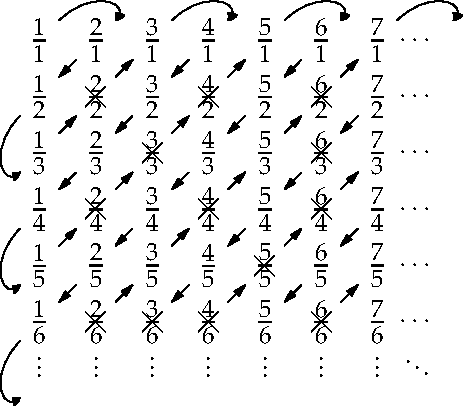
\includegraphics{cardinality-02-qcount}
	\end{minipage}
	\medbreak
	which identifies the negative rationals with $\Z^-$. By Theorem \ref{thm:zcount}, we deduce that $\nm{\Q}=\nm{\Z}=\aleph_0$.
\end{proof}


\goodbreak


Other countably infinite sets \emph{appear} to be even larger than $\Q$! For example:
\begin{itemize}
  \item Cartesian products such as $\Q\times\Q$.
  \item The \emph{algebraic numbers} $\mathbb{A}=\bigl\{x\in\C:p(x)=0\text{ for some polynomial $p$ with integer coefficients}\bigr\}$.\par
  Every rational number is algebraic ($\frac ab$ is a root of $p(x)=bx-a$), but so are many irrationals ($\sqrt 2$ is a root of $p(x)=x^2-2$). Non-algebraic numbers (e.g., $\pi$ and $e$) are termed \emph{transcendental.}
\end{itemize}

Arguments for these examples are left to the exercises.


\boldsubsubsection{The Least Infinite Cardinal?}

We introduced $\aleph_0$ to represent the cardinality of the `simplest' infinite set $\N$. Here is a compelling reason why the natural numbers should indeed be considered the \emph{most simple} infinite set.

\begin{thm}{}{finitealeph}
	$A$ is finite if and only if $\nm A<\aleph_0$.
\end{thm}

Otherwise said, every infinite set has cardinality \emph{at least as large} as the natural numbers: $\aleph_0$ may therefore be considered the least infinite cardinal.

\begin{proof}
	\begin{description}
		\item[\normalfont ($\Rightarrow$)]
		Express the set in roster notation $A=\{a_1,\ldots,a_n\}$. We must prove two things:\footnotemark{}
		\begin{description}
			\item[\normalfont($\nm A\le\aleph_0$)] Define $f:A\to\N$ by $f(a_k)=k$ for each $k\in\{1,2,3,\ldots,n\}$. This is injective since the distinct elements $a_k$ of $A$ map to distinct integers.
			\item[\normalfont($\nm A\neq\aleph_0$)] We show there are no bijections $\N\to A$. Suppose $g:\N\to A$ and consider the set
			\[
				g\bigl(\{1,\ldots,n+1\}\bigr)=\bigl\{g(1),\ldots,g(n+1)\bigr\}\subseteq A
			\]
			Since $A$ has $n$ elements, at least two of the values $g(1),\ldots,g(n+1)$ must be equal. Therefore $g$ is not injective and consequently not bijective.
		\end{description}
		\item[\normalfont ($\Leftarrow$)] See Exercise \ref{exs:finitealephproof}. \qedhere
	\end{description} 
\end{proof}

\footnotetext{%
	The $n=0$ case ($A=\emptyset$) works, though it feels strange: $f=\emptyset$ is a suitable injective (!) function $f:\emptyset\to\N$, and there are no functions $g\subseteq\N\to\emptyset$. It will help to think about the formal definition of \emph{function} (Section \ref{sec:func2})!%
}

We'll address the existence of infinite sets with cardinality \emph{larger} than $\aleph_0$ in the next section.

% \begin{aside}{}{}
% {\bf $\aleph_0$ versus $\infty$: what's the difference?}
% 
% It can be difficult to grasp why $\aleph_0$ and $\infty$ are not the same thing. The problem is compounded by references to an `infinite number' of objects whenever the cardinality of a set is not finite. This loose phrase is commonly used, but risks conflating the concepts of `infinite set' and `infinity.'\\
% So what is the difference between $\aleph_0$ and $\infty$? If there aren't an `infinite number' of natural numbers, how many are there? Theorem \ref{thm:finitealeph} says that $\aleph_0$ is `larger than any natural number.' Is this not what we mean by infinity? The reason we need a new symbol $\aleph_0$, and why it and $\infty$ are different, is twofold:
% \begin{enumerate}
% \item As we shall see shortly, there are infinite sets with greater cardinality than $\aleph_0$: in a naïve sense, there are multiple infinities. The single symbol $\infty$ is insufficient to distinguish sets with different infinite cardinalities.
% \item More philosophically, $\aleph_0$ is an \emph{object} in its own right; an object to which the cardinality of some set may be equal. Indeed, by Theorem \ref{thm:cardequiv}, $\aleph_0$ is an equivalence class.
% 
% By contrast, $\infty$ is typically not an object. The symbol $\infty$ is mostly used in \emph{interval notation} and when talking about \emph{limits:} in neither case does the symbol represent an object. For example:
% \begin{itemize}
%   \item The interval $(2,\infty)$ is the set of all real numbers greater than 2. We don't say `greater than 2 and \emph{less than infinity.}'
%   \item $\lim\limits_{x\to 3}\frac 1{(x-3)^2}=\infty$ means that the function $f(x)=\frac 1{(x-3)^2}$ gets unboundedly larger as $x$ approaches 3. It is incorrect to say that $f(x)$ `approaches infinity.' It is even worse to write $f(3)=\frac 1{(3-3)^2}=\infty$.
% \end{itemize}
% \end{enumerate}

%  The challenge of Cantor's notion of cardinality is to appreciate that the question, `How many natural numbers are there?' is meaningless!
% \end{aside}


\begin{exercises}{}{}
	A reading quiz and practice question can be found \href{http://www.math.uci.edu/~ndonalds/math13/selftest/8-1-cantor.html}{online}.
	
	\begin{enumerate}
	  \item Refresh your proof skills by proving explicitly that the following functions are bijections:
	  \begin{enumerate}
	    \item $g:\N\to\N_{\ge 2}:n\mapsto n+1$\qquad\qquad (b) \ $h:\N\to 2\N:n\mapsto 2n$
	  \end{enumerate}
  
  
		\item Prove that $\Z_{\ge -3}$ is countably infinite by constructing a bijective function $g:\N\to\Z_{\ge -3}$.
		
		
		\item Prove that the set $3\Z+2=\{3n+2:n\in\Z\}$ is countably infinite.
		
	
		\item Show that the set of all triples of the form $(n^2,5,n+2)$ with $n\in 3\Z$ is countably infinite by providing an explicit bijection with a known countably infinite set.
		
		\item\label{exs:easyintervalcard} State a bijection $g:(0,1)\to (4,6)$ which shows that these intervals have the same cardinality.
		
		\goodbreak

	
		\item Prove Lemma \ref{lemm:cardequiv} \ (\emph{revisit Theorem \ref{thm:compinjsurj} on the composition of bijective functions.})
		
		
		\item Prove that $A\subseteq B\Longrightarrow \nm A\le\nm B$ \ (\emph{show there exists an injective function $f:A\to B$}).
	
	
		\item\begin{enumerate}
		  \item Prove that $\N\times\N$ is countably infinite by modifying the proof of Theorem \ref{thm:qcount}.
			\item Combine part (a) with Theorem \ref{thm:qcount} to prove that $\Q\times\Q$ is countably infinite.
			\item\label{ex:cardunion} Suppose $A_n$ is countably infinite for each $n\in\N$ and list elements as follows:
		\begin{gather*}
			A_1=\{a_{11},a_{12},a_{13},a_{14},\ldots\}\\
			A_2=\{a_{21},a_{22},a_{23},a_{24},\ldots\}\\
			A_3=\{a_{31},a_{32},a_{33},a_{34},\ldots\},\ \ \text{etc.}
		\end{gather*}
		Prove that $\bigcup A_n$ is countably infinite \ (\emph{a countable union of countable sets is countable}).
		\end{enumerate}
	

		\bigskip

		\hspace{-\leftmargini}{Warning! The remaining exercises are significantly trickier.}
  
		\item Suppose $A\neq\emptyset$. Prove that $\nm A\le \nm B$ if and only if there exists a surjective function $g:B\to A$.\par
		(\emph{Hint: Use $g$ to construct an injective $f:A\to B$, and vice versa})
		
			
		\item \label{exs:algcard} Let $\mathbb A=\bigl\{x\in\C:p(x)=0\text{ for some polynomial $p$ with integer coefficients}\bigr\}$ be the set of \emph{algebraic} numbers. We prove that $\mathbb A$ is countably infinite.
	\begin{enumerate}
	    \item Let $M\in\N$. Prove that there are only finitely many choices of $d\in\N$ and $a_0,\ldots,a_d\in\Z$ such that $M=d+\nm{a_0}+\cdots +\nm{a_d}$.
	    \item Let $P_M=\bigl\{a_dx^d+\cdots +a_1x+a_0:d+\nm{a_0}+\cdots +\nm{a_d}=M\bigr\}$. Explain why $P_M$ is finite.
	    \item Show that $R_M=\bigl\{x\in\C:p(x)=0\text{ for some } p\in P_M\bigr\}$ is finite by using the fact that a degree $d$ polynomial has at most $d$ roots.
	    \item Prove that $\mathbb A=\bigcup_{M\in\N}R_M$ and conclude that $\mathbb A$ is countably infinite.
	\end{enumerate}
		
		
		\item\label{exs:finitealephproof} We complete the proof of Theorem \ref{thm:finitealeph}: if $\nm A<\aleph_0$, then $A$ is a finite set.\par
		We prove by contradiction. Suppose $A$ is infinite and that $\nm A<\aleph_0$. Then there exists an injective function $f:A\to\N$. List the range of $f$ in \emph{increasing} order:
		\[
		  \range(f)=\{n_1,n_2,n_3,\ldots\}\qquad n_1<n_2<n_3<\cdots
		\]
		\begin{enumerate}
		  \item Show that for all $k\in\N$, there exists a unique $a_k\in A$ satisfying $f(a_k)=n_k$.
		  \item Define $g:\N\to A$ by $g(k)=a_k$. Prove that $g$ is a bijection and hence obtain a contradiction.
		\end{enumerate}
	
		
		\item\label{exs:cardinf1} Suppose $C$ is countably infinite and let $c\in C$.
		\begin{enumerate}
			\item Show that there exists a bijection $h:\N\to C$ with $h(1)=c$.
		  \item Prove that $D=C\setminus\{c\}$ is countably infinite.\par
			(\emph{Hint: $h$ be as in part (a) and use $g$ from Example \ref{ex:easycantor} to construct $k:\N\to D$})
		\end{enumerate}
		
		
		\item\label{exs:cardinf2}
		\begin{enumerate}
		  \item Suppose $\nm A\ge\aleph_0$. Show that there exists $C\subseteq A$ for which $\nm C=\aleph_0$.
		  \item Prove that a set $A$ is infinite if and only if it has a proper subset $B$ with $\nm B=\nm A$.\par
		  (\emph{Hint: use part (a) and Exercise \ref{exs:cardinf1}})
		\end{enumerate}
		
		\item\label{exs:openclosedcard} Describe an \emph{explicit} bijection $g:[0,1]\to (0,1)$, and thus demonstrate that the intervals have the same cardinality.\par
		(\emph{Hint: $\{\frac 1n:n\in \N_{\ge 2}\}$ is a countably infinite subset of $(0,1)$})
		
	\end{enumerate}

\end{exercises}

\clearpage



\subsection{Uncountable Sets}\label{sec:uncountable}

Since $\Q$ seems so large, you might imagine that no sets could have strictly larger cardinality. But we haven't yet thought about the real numbers\ldots

\begin{defn}{}{}
	A set $A$ is \emph{uncountable} if $\aleph_0<\nm A$. Otherwise said, there exists an injection $f:\N\to A$ but no bijection $g:\N\to A$.
\end{defn}

\begin{thm}{}{intervaluncount}
	The interval $(0,1)$ of real numbers is uncountable.
\end{thm}

We denote the cardinality of the interval $(0,1)$ by $\fc$ for \emph{continuum.} The theorem may therefore be written $\aleph_0<\fc$. We prove by showing that $\aleph_0\le\fc$ and $\aleph_0\neq\fc$.

\begin{proof}
	\begin{description}
		\item[\normalfont ($\aleph_0\le\fc$)] The function $f:\N\to(0,1):n\mapsto \frac 1{n+1}$ is plainly injective:
		\[
			f(n)=f(m)\implies \frac 1{n+1}=\frac 1{m+1}\implies n=m
		\]
		\item[\normalfont ($\aleph_0\neq\fc$)] Suppose, for contradiction, that $g:\N\to(0,1)$ is a bijection. Express the sequence of values $g(1)$, $g(2)$, $g(3),\ldots$ as decimals:\footnotemark
		\[
			\begin{array}{c}
				g(1)=0.\textcolor{blue}{b_{11}}b_{12}b_{13}b_{14}b_{15}b_{16}\cdots\\[2pt]
				g(2)=0.b_{21}\textcolor{blue}{b_{22}}b_{23}b_{24}b_{25}b_{26}\cdots\\[2pt]
				g(3)=0.b_{31}b_{32}\textcolor{blue}{b_{33}}b_{34}b_{35}b_{36}\cdots\\[2pt]
				g(4)=0.b_{41}b_{42}b_{43}\textcolor{blue}{b_{44}}b_{45}b_{46}\cdots\\[2pt]
				g(5)=0.b_{51}b_{52}b_{53}b_{54}\textcolor{blue}{b_{55}}b_{56}\cdots\\[-2pt]
				\vdots\\[-5pt]
			\end{array}
			\qquad
			\text{where each }b_{ij}\in\{0,\ldots,9\}
		\]
		Define a new decimal
		\[
			x:=0.x_1x_2x_3x_4x_5\cdots \in (0,1)\qquad\text{where}\quad x_n=
			\begin{cases}
				1&\text{if }\textcolor{blue}{b_{nn}}\neq 1\\
				2&\text{if }\textcolor{blue}{b_{nn}}=1
			\end{cases}
		\]
		Since $x$ disagrees with $g(n)$ at the $n\th$ decimal place, we see that $x\neq g(n)$: that is, $x$ is \emph{not} in the above list. However $x\in(0,1)$ and $g$ is surjective, so $x$ \emph{must} be in the list: contradiction.\qedhere
	\end{description}
\end{proof}

\footnotetext{%
	\label{fn:decimalcantor}A number $x\in(0,1)$ has two decimal representations if and only if one of them terminates and the other ultimately becomes an infinite sequence of 9's: e.g., $0.135=0.1349999\ldots$. For this proof, we choose the terminating decimal whenever it exists. We restrict to $x_n=1,2$ later in the proof to keep away from these double representations.%
}

The second part of the proof is known as \emph{Cantor's diagonal argument,} since we compare the constructed decimal $x$ with the \textcolor{blue}{diagonal} of an infinite square of integers. Since the interval $(0,1)$ is uncountable, and $(0,1)\subseteq\R$, it is immediate that the real numbers are also uncountable. Using only the ideas developed so far (a combination of Exercises \ref*{sec:cantor}.\ref{exs:easyintervalcard} and \ref{exs:openclosedcard}), we could prove directly that every interval of finite length has cardinality $\fc$. It is easier, however, to delay this momentarily\ldots\smallbreak


Even more amazingly, Cantor's middle-third set (Example \ref{ex:cantorthird}) also has cardinality $\fc$, despite seeming vanishingly small! The details, and more, are in Exercise \ref{exs:middlethirdcard}.


\goodbreak


\boldsubsubsection{Non-explict Comparison of Cardinalities}

%Our discussion thus far is merely scratching the surface of a truly weird subject. We conclude these notes with a couple more ideas.\smallbreak

The following result is very useful for comparing cardinalities. %It allows us to prove that two sets have the same cardinality \emph{without} explicitly constructing bijective functions. Injective functions are usually much easier to find.

\begin{thm}{Cantor--Schröder--Bernstein}{}
	If $\nm A\le\nm B$ and $\nm B\le\nm A$, then $\nm A=\nm B$.
\end{thm}

This seems like it should be obvious, but pause for a moment: it is \emph{not} a result about \emph{numbers!} The theorem should be understood in the context of Definition \ref{defn:infcard}, in which language it becomes:
\[
	\tcbhighmath{
		\text{%
			If there exist \emph{injections} $f:A\to B$ and $g:B\to A$, then there exists a \emph{bijection} $h:A\to B$
		}
	}
\]

The proof is beautiful, though a little long to reproduce here; if you're interested, check out any elementary text on set theory. Its usefulness is that it allows us to equate cardinalities without explicitly constructing \emph{bijective} functions; \emph{injective} functions are typically easier to conjure!


\begin{example}{}{}
	The following functions are both injective (\emph{only}---they are not bijective!):
	\begin{gather*}
		f:(0,1)\to[0,1]:x\mapsto x \tag{$\range(f)=(0,1)\subsetneq[0,1]$}\\
		g:[0,1]\to (0,1):x\mapsto \frac 12x+\frac 14 \tag{$\range(g)=[\tfrac 14,\tfrac 34]\subsetneq(0,1)$}
	\end{gather*}
	By Cantor--Schröder--Bernstein, the sets $(0,1)$ and $[0,1]$ have the same cardinality ($\fc$). Note how fast this was; we didn't have to construct an explicit bijection $h:(0,1)\to[0,1]$, a much nastier business (see Exercise \ref*{sec:cantor}.\ref{exs:openclosedcard})
\end{example}


As recently advertised, this example generalizes to cover all intervals.

\begin{cor}{}{intervalcard}
	All intervals (of positive length) have cardinality $\fc$.
\end{cor}

\begin{proof}
	Let $A$ be an interval (could be infinite length) and choose a subinterval $(a,b)\subseteq A$. The following functions are \emph{injective}:\par
	\begin{minipage}[t]{0.6\linewidth}\vspace{0pt}
		\begin{itemize}
	  	\item $f:(0,1)\to A$ where $f(x)=a+(b-a)x$; this maps $(0,1)$ onto $\range(f)=(a,b)\subseteq A$.
	  	\item $\iota:A\to\R$ where $\iota(x)=x$.
	  	\item $g:\R\to(0,1)$ where $g(x)= \frac 12+\frac 1\pi\tan^{-1}x$; this is in fact bijective with inverse $g^{-1}(y)=\tan\bigl(\pi y-\frac\pi 2\bigr)$.
		\end{itemize}
	\end{minipage}
	\hfill
	\begin{minipage}[t]{0.39\linewidth}\vspace{0pt}
		\hfill
		\begin{tabular}{@{}c@{}}
			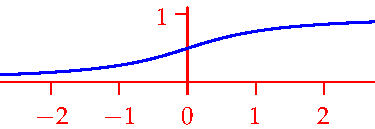
\includegraphics{cardinality-03-tan}
			\\
			\textcolor{blue}{$g(x)=\frac 12+\frac 1\pi\tan^{-1}x$}
		\end{tabular}
	\end{minipage}
	\bigbreak
	Putting everything together:
	\[
		\smash[t]{\nm{(0,1)}\overset{f}{\le}
		\nm A\overset{\iota}{\le}
		\nm\R \overset{g}{=}\nm{(0,1)}}
	\]
	By Cantor--Schröder--Bernstein, all these sets have the same cardinality, namely $\fc$.
\end{proof}

Further examples can be found in the exercises.

\vfil\goodbreak


\boldsubsubsection{Cantor's Paradoxical Theorem}

For a final punchline, we generalize Theorem \ref{thm:powercard} which, for finite sets $A$, asserted that $\nm{\cP(A)}=2^{\nm A}$ is \emph{strictly larger} than $A$ itself. We now have the technology to attack this for \emph{infinite} sets.

\begin{thm}{Cantor}{}
	If $A$ is any set, then $\nm A\lneq\nm{\cP(A)}$.
\end{thm}

The main implication is that \emph{there is no largest cardinality!} We can always construct a set with strictly larger cardinality just by taking the power set. For example, $\nm{\cP(\R)}>\nm\R=\fc$. Want an even larger cardinality? Try $\cP\bigl(\cP(\R)\bigr)$, or $\cP\bigl(\cP(\cP(\R))\bigr)$! This process may be continued indefinitely.

\begin{proof}
	If $A=\emptyset$, the result is trivial. Otherwise, first observe that $f:a\mapsto\{a\}$ defines an injective function $f:A\to\cP(A)$, whence $\nm A\le\nm{\cP(A)}$.\smallbreak
	To complete the argument we must show that no \emph{bijective} function $g:A\to\cP(A)$ can exist. Suppose, for a contradiction, that $g:A\to\cP(A)$ is bijective, and consider the set 
	  \[
	  	X=\bigl\{a\in A:a\notin g(a)\bigr\} \tag*{\phantom\qedhere}
	  \]
\end{proof}

Take stock for a moment and \emph{think} about $X$. Since $g(a)$ is a \emph{subset} of $A$, the condition $a\not\in g(a)$ is legitimate, whence $X$ is a genuine subset of $A$ ($X\in\cP(A)$). A simple example will hopefully help.
  
\begin{example}{}{cantorproof}
	Let $A=\{1,2,3\}$ and define a function $g:A\to\cP(A)$ by
  \[
  	g(1)=\{1,2\},\qquad g(2)=\{1,3\},\qquad g(3)=\emptyset
  \]
  Since $1\in g(1)$, \ $2\notin g(2)$, and $3\notin g(3)$, we see that $X=\{2,3\}$. Since our goal is to prove that no \emph{bijection} $A\to\cP(A)$ can exist, it is important to note that this $g$ is \emph{not bijective}; indeed $g$ isn't surjective, since $X\notin\range(g)=\bigl\{\{1,2\},\{1,3\},\emptyset\bigr\}$. This last observation is what finishes the proof\ldots
\end{example}

\begin{proof}[Proof Continued]  
	By assumption, $g$ is \emph{surjective}. Thus $X\in\range(g)$. Otherwise said, $X=g(a)$ for some $a\in A$. We ask whether this \emph{element} $a$ lies in the \emph{set} $X$:
	\begin{align*}
		a\in X&\iff a\notin g(a)\tag{definition of $X$}\\
		&\iff a\notin X\tag{since $X=g(a)$}
	\end{align*}
	The conclusion $a\in X\Longleftrightarrow a\notin X$ is plainly a contradiction! No bijection $g:A\to\cP(A)$ can exist, and so $\nm A\lneq\nm{\cP(A)}$.
\end{proof}

Cantor's theorem played a key role in pushing set theory towards axiomatization, in part because of a simple paradox. If a `set' is merely a collection of objects, we may consider the `set of all sets' $S$. Its power set $\cP(S)$ is a set of sets, which must be a subset of $S$. Plainly $\nm{\cP(S)}\le\nm S$; but this contradicts Cantor's theorem!\smallbreak

The remedy is a rigorous definition of `set.' \emph{Axiomatic set theory} describes a small number of legitimate ways to build sets, of which we've seen several in these notes: e.g., union, power set, set-builder notation. In particular, the `set of all sets' \emph{cannot} be legitimately constructed.\footnote{%
	The critical condition for preventing Cantor's paradox is that set-builder notation $\{x\in A:P(x)\}$ can only produce a subset of an \emph{already existing} set $A$. The `set of all sets' would have the form $\{x:P(x)\}$ where $x$ is \emph{unrestricted}.%
}  



\boldsubsubsection{Some Final Thoughts on the Limits of Proof}

During this course we've learned some of the basic methods and concepts used by mathematicians. In particular, we've learned how to use proofs to demonstrate the truth of statements about mathematical objects. As we finish, it makes sense to reflect on the limits of our methods.\smallbreak

By the early 20\th{} century, the discovery of various paradoxes and contradictions (such as  Cantor's) caused a foundational crisis in mathematics. If a concept as basic as \emph{set} is self-contradictory, how are we to have faith in any mathematical conclusion?! The response to this crisis was an effort to formulate a list of reasonable axioms from which all mathematics could be derived using basic logical reasoning. Such an axiomatic foundation would ideally satisfy two conditions:
\begin{itemize}\itemsep0pt
  \item \emph{Consistency}:\lstsp No contradiction can be derived from the axioms.
  \item \emph{Completeness}:\lstsp All true mathematical statements could be derived from the axioms.
\end{itemize}
Any hope for such a foundation was crushed in 1931, when Kurt Gödel published his famous \emph{Incompleteness Theorems}, showing that no such axiomatic system could exist. Very roughly, Gödel showed that in any consistent axiomatic system strong enough to produce some basic arithmetic, there are \emph{undecideable} statements; neither deducible nor refutable from the axioms. Perhaps even worse, no such system can prove its own consistency.\smallbreak

While the strongest aims of early 20\th{} axiomatics cannot be accomplished, contemporary research was able to provide a foundation that most modern mathematicians deem adequate. The most popular approach is to base all of mathematics on \emph{set theory}---as your studies progress, you'll see that many of the objects you study can be formalized as sets together with functions and relations between them. We've started this work already: Chapter \ref{chap:relations} says that functions and relations are themselves sets! Numbers like 0, 1, 2, $\frac{12}{19}$ or even $\pi=3.14\ldots$ can be thought of as sets if one so desires. In turn, set theory is often axiomatized using the ZFC axioms (short for Zermelo--Fraenkel set theory with the Axiom of Choice).\smallbreak

While the ZFC system remains subject to Gödel's limitations,\footnote{%
	Perhaps the most famous undecidable statement in ZFC is relevant to our recent discussion: the \emph{continuum hypothesis} is the claim that no set has cardinality strictly between $\aleph_0$ and $\fc$; that intervals are the simplest (`smallest') uncountable sets.%
} it has proven able to formalize most of the mathematics actually used by current mathematicians, and has not (thus far!) produced any inconsistencies. While there is plenty of fun to be had exploring set theory, its history and its quirks, most modern mathematicians feel little need to dwell on the foundational issues of last century!


% \begin{proof}
% We are assuming that we have two distinct, injective functions $f:A\to B$ and $g:B\to A$. We must construct a bijective $h:A\to B$.
% 
% Consider some $\alpha\in A$. Does $\exists\beta\in B$ such that $\alpha=g(\beta)$? If so, then the injectivity of $g$ says that $\beta$ is unique and we might as well write $\beta=g^{-1}(\alpha)$. Now suppose that $\exists\gamma\in A$ such that $\beta=f(\gamma)$. Again, if $\gamma$ exists, the injectivity of $f$ says it is unique and we can write $\gamma=f^{-1}(\beta)=f^{-1}(g^{-1}(\alpha))$.
% 
% Starting with $\alpha\in A$, we ask how far we can continue this process of following the functions $g,f$ in reverse. Each $\alpha\in A$ must be one of two possible types:
% \begin{enumerate}
%   \item Type I: The process continues indefinitely, or will terminate in the set $A$: i.e. after an even number of steps, the chain results in some $a\in A$ which is \emph{not} in the image of $g$ and thus for which $g^{-1}(a)$ does not exist.
%   \item Type II: The process terminates in the set $B$.
% \end{enumerate}
% We now define the function that will turn out to be the required bijection: if $\alpha\in A$, define
% \[h(\alpha)=\begin{cases}
% f(\alpha)&\text{if $\alpha$ Type 1},\\ 
% g^{-1}(\alpha)&\text{if $\alpha$ Type 2}.
% \end{cases}\]
% 
% Is $h$ a well-defined function? There is no overlap between the two Types. Furthermore, if $\alpha$ is Type I, $f(\alpha)$ is always defined, while for Type 2, the we must be able to apply $g^{-1}$ at least once to $\alpha$. $h:A\to B$ is therefore well-defined.
% 
% We now prove that $h$ is a bijection.
% 
% Suppose $h(\alpha_1)=h(\alpha_2)$. There are three cases:
% \begin{enumerate}
% \item $\alpha_1,\alpha_2$ of Type 1. Then the injectivity of $f$ forces, 
% \[h(\alpha_1)=h(\alpha_2)\implies f(\alpha_1)=f(\alpha_2)\implies\alpha_1=\alpha_2.\]
% \item $\alpha_1,\alpha_2$ of Type 2. Then we apply $g$ to obtain, 
% \[h(\alpha_1)=h(\alpha_2)\implies g^{-1}(\alpha_1)=g^{-1}(\alpha_2)\implies\alpha_1=\alpha_2.\]
% \item $\alpha_1$ of Type 1 and $\alpha_2$ of Type 2. Then, 
% \[h(\alpha_1)=h(\alpha_2)\implies f(\alpha_1)=g^{-1}(\alpha_2)\implies \alpha_2= 
% g(f(\alpha_1).\]
% But this says that $\alpha_1$ and $\alpha_2$ have the same type. A contradiction.
% \end{enumerate}
% $h$ is therefore injective.\\
% 
% Now for surjectivity. Let $\beta\in B$. We want to find an $\alpha$ with $h(\alpha)=\beta$. Consider 
% the chain of $g(\beta)$. If $g(\beta)$ is of Type 1 then $f^{-1}(\beta)$ is well-defined and $h(f^{-1}(\beta))=\beta$. If instead $g(\beta)$ is of Type 2 then $h(g(\beta))=g^{-1}(g(\beta))=\beta$. Hence $h$ is onto.
% \end{proof}

\begin{exercises}{}{}
	A reading quiz and practice question can be found \href{http://www.math.uci.edu/~ndonalds/math13/selftest/8-2-uncountable.html}{online}.

	\begin{enumerate}
	  \item Decide the cardinality of each set. No working is necessary.
	  \begin{enumerate}
	    \item $\N_{\le 12}$\hfill (b) \ $\Z_{\le 12}$\hfill (c) \ $(0,5]$\hfill 
	    (d) \ $[2,\pi]\cap\Q$\hfill (e) \ $\cP\bigl(\{\R\}\bigr)$ \hfill 
	    (f) \ $\bigcap\limits_{x\in\R^+}[3-\frac 1x,3+\frac 1x)$
	  \end{enumerate}
	  
	  
	  \item Find \emph{explicit} bijections (thus showing that the given intervals have the same cardinality):
	  \begin{enumerate}
	    \item $f:[2,3)\to [1,5)$ \qquad (b) \ $g:[2,3)\to (1,5]$\qquad 
	    (c) \ $h:(-3,2)\to\R$ \qquad (d) \ $j:\R\to(1,\infty)$
	  \end{enumerate}
	  (\emph{Hint: The proof of Corollary \ref{cor:intervalcard} should provide some inspiration---be creative}) 
  
  
  	\item Let $B=[3,5)\cup(6,10)$. Use the Cantor--Schröder--Bernstein Theorem to prove that $\nm B=\fc$.\par
  	(\emph{Hint: State injective functions $f:(0,1)\to B$ and $g:B\to(0,1)$})
  	
  	
  	\goodbreak
  	
  	
  	\item\begin{enumerate}
  		\item Prove that $f:\N\times\N\to\N$ defined by $f(m,n)=2^m3^n$ is injective.
  		\item Use part (a) and the Cantor--Schröder--Bernstein Theorem to conclude that $\nm{\N\times\N}=\aleph_0$.
  		\item Extend your argument to prove that, for any natural number $k$,	\smash{$|\!\underbrace{\N\times\cdots\times\N}_{k\text{ times}}\!|=\aleph_0$}
  		\item Use part (b) to give an alternative proof that $\nm{\Q^+}=\aleph_0$.
  	\end{enumerate}
  	
  
	  \item Revisit the proof of Cantor's Theorem, and Example \ref{ex:cantorproof}.
	  \begin{enumerate}
	    \item Suppose $g:\{1,2,3,4\}\to\cP(\{1,2,3,4\})$ is defined by
	  	\[
	  		g(1)=\{2,3\},\qquad g(2)=\{1,2\},\qquad g(3)=\emptyset,\qquad g(4)=\{1,2,4\}\]
	  	Compute the set $X=\bigl\{a\in\{1,2,3,4\}:a\not\in g(a)\bigr\}$.
	  	\item Repeat part (a) for $g:\N\to\cP(\N):n\mapsto\{x\in 2\N:x\le n\}$.\par
	  	(\emph{Hint: Try some examples first! What is $g(1)$? Is $1\in g(1)$? What about $2\in g(2)$?})
	  \end{enumerate}
  
  
	  \item Let $\mathbb I=\R\setminus\Q$ be the set of irrational numbers.
		\begin{enumerate}
		  \item Prove that $\nm{\mathbb I}\le\fc$.
		  \item Prove that $x\in\N\implies x+\sqrt 2\in\mathbb I$. Hence conclude that $\aleph_0\le\nm{\mathbb I}$.
		  \item Argue that the irrational numbers are uncountable \ ($\nm{\II}=\fc$ is harder to show).
		  \item Show that the \emph{transcendental} (non-algebraic) numbers are uncountable (see Exercise \ref*{sec:cantor}.\ref{exs:algcard}).
	 	\end{enumerate}
 	
 	
  	\item Give an example of an uncountable set $I$ and an indexed collection $\{A_n:n\in I\}$ for which all the following conditions hold:
		\begin{itemize}
		  \item Each $A_n$ is countably infinite.
    	\item If $m \neq n$, then $A_m \neq A_n$.
    	\item For all $m,n$, either $A_m \subseteq A_n$ or $A_m \supseteq A_n$.
    	\item $\bigcup_{n \in I} A_n$ is countably infinite.
		\end{itemize}
 	
 	
   	\item The proof of Cantor's Theorem makes use of a construction similar to \emph{Russell's paradox.} Let $X$ be the `set' of all sets which are not members of themselves:
  	\[
  		X=\{A:A\not\in A\}
  	\]
  	\begin{enumerate}
    	\item Suppose $X$ is a set. By asking yourself if $X$ is a member of itself, deduce a contradiction.\par
    	(\emph{The point of Russell's paradox is that objects like $X$ cannot be considered sets!})
    	\item Russell's paradox is one version of an ancient logical conundrum with many guises. E.g.,
    	\begin{quote}
    		A town has one barber, who cuts the hair of all townspeople, and only those people, who do not cut their own hair: Who cuts the barber's hair?
    	\end{quote}
    	Can you explain the connection between this and Russell's paradox?
  	\end{enumerate}
  	
  
		\item In Exercise \ref*{sec:indexed}.\ref{exs:cantorset}, we saw that Cantor's middle-third set $\mathcal C$ is the set of all numbers in $[0,1]$ possessing a ternary expansion consisting only of 0's and 2's. By modifying the proof of Theorem \ref{thm:intervaluncount}, argue that $\mathcal C$ is uncountable.\par
		(\emph{Exercise \ref{exs:middlethirdcard} establishes the stronger result $\nm{\mathcal C}=\fc$})
  
  
  	\goodbreak
  	
  	
  	\item[]The remaining questions are more of a challenge: if these seem interesting, consider taking a set theory course!
  	
  	
  	\item Express a real number $x\in(0,1)$ as a decimal $x=0.x_1x_2x_3x_4\ldots$	where we choose the terminating decimal whenever there is a choice (footnote \ref{fn:decimalcantor}). Prove that
  	\[
  		f:(0,1)\times (0,1)\to (0,1)
  		\quad\text{defined by}\quad
  		f(x,y)=0.x_1y_1x_2y_2x_3y_3\ldots
  	\]
  	is \emph{injective}. Hence conclude that $\nm{\R^2}=\fc$.
		
  
		\item\label{exs:charfunc} If $A$ and $B$ are non-empty sets we let $A^B$ denote the set of all \emph{functions} $f:B\to A$.
		\begin{enumerate}
	    \item If $A=\{0,1\}$ and $B=\{a,b,c\}$, list all elements of $A^B$. What is $\nm{A^B}$?
	    \item If $A$ and $B$ are finite sets, show that $\nm{A^B} = \nm{A}^{\nm B}$.
	    \item Let $B$ be a set and $Y\subseteq B$. The \emph{characteristic function} of $Y$ is $\chi_Y:B\to\{0,1\}$  where
	    \[
	    	\chi_Y(x)=
	    	\begin{cases}
	        1 &\text{if } x\in Y\\
	        0 &\text{if } x\notin Y
	      \end{cases}
	    \]
	    Prove that $\Phi:\cP(B)\to\{0,1\}^B$ defined by $\Phi(Y)=\chi_Y$ is \emph{bijective}.\par
	    (\emph{If $B$ is finite, this provides another proof that $\nm{\cP(B)} = 2^{\nm B}$})
		\end{enumerate}

  		
		\item\label{exs:middlethirdcard} Let $x\in[0,1]$. A \emph{binary expansion} of $x$ is a sequence $(b_n)$ of zeros and ones such that
	  \[
	  	x=\sum_{n=1}^\infty \frac{b_n}{2^n}
	  \]
	  The binary expansion of $x\in[0,1]$ is (almost) unique;\footnotemark{} if there is a choice, take the terminating expansion. Define a function $f:[0,1]\to\cP(\N)$ (the set of subsets of $\N$) by
	  \[
	  	f(x)=\{n\in\N:b_n=1\text{ in the binary expansion of $x$}\}
	  \]
	  \begin{enumerate}
	    \item Prove that $f$ is injective, and that, consequently, $\fc\le\nm{\cP(\N)}$.
	    \item Is $f$ surjective?\par
	    (\emph{Hint: consider the set $X=\{2,3,4,\ldots\}\in\cP(\N)$})
			\item Let $\mathcal C$ be Cantor's middle-third set. Prove that $g:\cP(\N)\to\mathcal C$ is a bijection, where
			\[
				g(X)=\sum\limits_{n\in X}^\infty\frac{2}{3^n}
			\]
			\item Use the Cantor--Schröder--Bernstein Theorem to conclude that $\nm{\cP(\N)}=\nm{\mathcal C}=\fc$.\par
			(\emph{Together with Exercise \ref{exs:charfunc}, this shows why we could write $\fc=2^{\aleph_0}$})
		\end{enumerate}

	\end{enumerate}

\end{exercises}

\footnotetext{%
	Binary expansions are unique unless $x$ has a terminating expansion, in which case the there is a second representation with an infinite string of 1's: e.g., $[0.011111\cdots]_2=[0.1]_2$. This discussion is beloved of computer scientists who, following Exercise \ref{exs:charfunc}, might view $\cP(\N)\sim\{0,1\}^\N$ as the set of \emph{binary sequences/strings} $(x_1,x_2,x_3,\ldots)$, where each $x_j\in\{0,1\}$.%
}
